%! Author = breandanconsidine
%! Date = 9/19/21

% Preamble
\documentclass[11pt]{article}

% Packages
\usepackage{amsmath}
\usepackage{hyperref}
\usepackage{amsfonts}
\usepackage{listings}
\usepackage{tikz}
\usepackage{amssymb}
\usetikzlibrary{matrix, positioning}
\newcommand*{\greysquare}{\textcolor{gray}{\blacksquare}}

% Document
\author{Instructor: Xujie Si, TA: Breandan Considine}
\date{Due: Oct. 10th before class}
\title{COMP 597: Assignment \#1}
\begin{document}
    \maketitle
    \noindent This is the first assignment of COMP 597: Automated Reasoning with ML.

    \section{Cryptography with SAT}

    The following solutions can be obtained using a solver of your choice. Please show all work. Only solutions obtained using a SAT solver will receive credit.\\

    % https://www.cs.rochester.edu/u/kautz/Courses/244autumn2008/Papers/cook-mitchell-1997.pdf
    \noindent \textbf{Emirpimes} (20 points): An \textit{emirp} is a prime whose digits, when reversed, produce a different prime. An \textit{emirpimes} is a semiprime whose reverse is a different semiprime, e.g., $11659567_{10}$. Confirm its prime factors are emirps in bases 2 and 10. Find another such number. What is the largest emirpimes you can find, whose prime factors are twin emirps in at least two bases?\\

    \noindent \textbf{Bonus} (10 points): A \textit{cryptarithm} is a cipher, $\varphi: \{A,\ldots, Z\}^*\leftrightarrow \{0, \ldots, 9\}^*$, alongside a meaningful string, whose ciphertext satisfies some equation, e.g.:

    \begin{lstlisting}[basicstyle=\scriptsize\ttfamily]
NINETEEN + THIRTEEN + THREE + TWO + TWO + ONE + ONE + ONE = FORTYTWO
42415114 + 56275114 + 56711 + 538 + 538 + 841 + 841 + 841 = 98750538
    \end{lstlisting}

    \noindent Construct a 20+-character cryptarithm parseable by the following grammar,
    \begin{align*}
E &\rightarrow A \mid \ldots \mid Z \mid EE \mid E O E \mid ( E )\\
O &\rightarrow + \mid \times \mid \div \mid -\footnotemark\\
S &\rightarrow E = E
    \end{align*}
    \footnotetext{Interpreted in the usual way, but additive and multiplicative identity are forbidden.}\noindent where $\texttt{eval}\big(\varphi(E)\big) = \texttt{eval}\big(\varphi(E')\big)$ and $\texttt{charset}(E) \neq \texttt{charset}(E')$. Every plaintext word should be defined in the English 10k dictionary.\footnote{\tiny\url{https://github.com/first20hours/google-10000-english/blob/master/google-10000-english.txt}} In order to receive credit, it must not be possible to find your cryptarithm (or algebraic rewritings thereof) on the internet or in other classmates' assignments.\\

    \pagebreak


    \section{Build or improve a SAT solver}

    \noindent \textbf{Programming exercise} (40 points): Please select one of the following two options, write a short report, and submit your source code. Please provide instructions for how reproduce your findings and a few test cases.

    \begin{enumerate}
        \item Write a SAT solver from scratch by implementing an existing algorithm such as DPLL, unit propagation or two-watched literals, describe your implementation and evaluate it on a few toy SAT problems.
        \item Make a substantive improvement to a competitive SAT solver (e.g. Kissat or MiniSat) which measurably increases performance on a standard benchmark, and document your approach and findings.
    \end{enumerate}

    % https://courses.cs.washington.edu/courses/cse599a2/15wi/
    \section {Uninterpreted function equivalence}

    \noindent \textbf{SMT exercise} (20 points): Show all work to receive full credit. Where required, typeset a proof sketch using \LaTeX, then translate the proof into your favorite SMT solver to construct a specific example or counterexample.

    \begin{enumerate}
        \item A polynomial equation whose coefficients and solutions are integers is called \textit{diophantine}. Let $w, x, y, z \in \mathbb{Z}$ and report your solver's largest nontrivial solutions to each of the following diophantine equations:\\ (a) $x^2+y^2+z = wxy$ (b) $w^3 + x^3 = y^3+z^3$ (c) $w^z + x^z = y^z + z$.
        \item Prove that $\mathbb{Z}^{n\times n}$ is associative over $\otimes$, and $\otimes$ is distributive over $\oplus$ for some large $n$. \textbf{Bonus} (5 points): Give an example of a nontrivial finite commutative semiring whose elements are matrices and prove it.
        \item A nonnegative matrix whose rows and columns all sum to the same number is called \textit{bistochastic}. Find distinct examples $M_1, M_2: \mathbb{Z}^{n\times n}$ for some large $n$ such that both are nontrivial bistochastic matrices. \textbf{Bonus} (5 points): Is $M_i M_j$ is bistochastic for all bistochastic $M_i, M_j$?
%        \item Consider the polynomial kernel $\Delta: (\mathbf{f}, \mathbf{g})\mapsto (\mathbf{f}\cdot\mathbf{g} + r)^q$. The \textit{kernel trick} states $\forall \mathbf{f}, \mathbf{g}: \mathbb{Z}^d$, $\exists \varphi \mid \langle\varphi(\mathbf{f}), \varphi(\mathbf{g})\rangle = \Delta(\mathbf{f}, \mathbf{g})$. Show the kernel trick holds by finding $\varphi$ for some large $r, d, q: \mathbb{N}$. What can we say about $\mathcal O(\langle\varphi, \varphi'\rangle)$ as $d, q \rightarrow \infty$? Is $\Delta$ a metric? Prove or disprove it.
        \item Prove that 1D discrete convolution, $*: (f, g)[x] \mapsto \sum_{s \in S}f[x-s]g[s]$, over $S=[-j, j]$ for some large value $j \in \mathbb{N}$ is translation equivariant. \textbf{Bonus} (10 points): Prove the 2D case for MNIST, i.e., $[0, 255]^{28\times 28}$.
    \end{enumerate}

    \noindent Only evidence in the form of (1) an example or counterexample, or (2) an interpretable proof will be accepted. Proofs should be \textit{constructive} where necessary. Encoding the problem and reporting UNSAT is not constructive.\pagebreak

    \section {Exploring the multiverse}
    \textbf{Creative coding} (20 points): Consider a multiverse $\mathcal{M}$, with some strange physical laws, whose dynamics are governed by the following eight rules.\\

        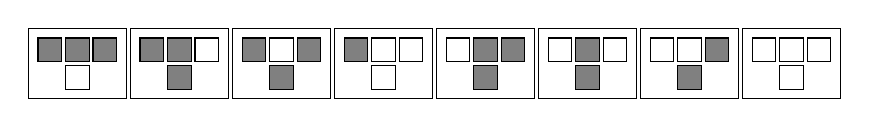
\begin{tikzpicture}[b/.style={draw, minimum size=3mm, fill=gray},w/.style={draw, minimum size=3mm},
            m/.style={matrix of nodes, column sep=1pt, row sep=1pt, draw}, node distance=1pt]
            \matrix (A) [m=0]{
                |[b]|&|[b]|&|[b]|\\
                &|[w]|\\
            };
            \matrix (B) [m=1, right=of A]{
                |[b]|&|[b]|&|[w]|\\
                &|[b]|\\
            };
            \matrix (C) [m=0, right=of B]{
                |[b]|&|[w]|&|[b]|\\
                &|[b]|\\
            };
            \matrix (D) [m=0, right=of C]{
                |[b]|&|[w]|&|[w]|\\
                &|[w]|\\
            };
            \matrix (E) [m=1, right=of D]{
                |[w]|&|[b]|&|[b]|\\
                &|[b]|\\
            };
            \matrix (F) [m=1, right=of E]{
                |[w]|&|[b]|&|[w]|\\
                &|[b]|\\
            };
            \matrix (G) [m=1, right=of F]{
                |[w]|&|[w]|&|[b]|\\
                &|[b]|\\
            };
            \matrix (H) [m=0, right=of G]{
                |[w]|&|[w]|&|[w]|\\
                &|[w]|\\
            };
        \end{tikzpicture}\\

    \noindent These rules describe a substitution system, in which the first row denotes a pattern match, and the second row denotes the subsequent state of the innermost cell. In this multiverse, the fabric of space folds in upon itself: travel far enough in any direction and you shall always return from whence you came. For example, we can visualize three steps in the time evolution of the universe $\mathcal{U}': \{\square,\greysquare\}^{16} \in \mathcal{M}$, starting from the initial state $t$ as follows:\\

    \noindent\begin{tabular}{ccc}
        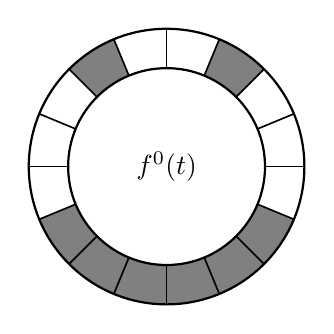
\begin{tikzpicture}[>=latex,font=\sffamily,semithick,scale=1.75]
        \fill [white] (0,0) -- (90.0:1) arc [end angle=67.5, start angle=90.0, radius=1] -- cycle;
        \fill [gray] (0,0) -- (67.5:1) arc [end angle=45.0, start angle=67.5, radius=1] -- cycle;
        \fill [white] (0,0) -- (45.0:1) arc [end angle=22.5, start angle=45.0, radius=1] -- cycle;
        \fill [white] (0,0) -- (22.5:1) arc [end angle=0.0, start angle=22.5, radius=1] -- cycle;
        \fill [white] (0,0) -- (0.0:1) arc [end angle=-22.5, start angle=0.0, radius=1] -- cycle;
        \fill [gray] (0,0) -- (-22.5:1) arc [end angle=-45.0, start angle=-22.5, radius=1] -- cycle;
        \fill [gray] (0,0) -- (-45.0:1) arc [end angle=-67.5, start angle=-45.0, radius=1] -- cycle;
        \fill [gray] (0,0) -- (-67.5:1) arc [end angle=-90.0, start angle=-67.5, radius=1] -- cycle;
        \fill [gray] (0,0) -- (-90.0:1) arc [end angle=-112.5, start angle=-90.0, radius=1] -- cycle;
        \fill [gray] (0,0) -- (-112.5:1) arc [end angle=-135.0, start angle=-112.5, radius=1] -- cycle;
        \fill [gray] (0,0) -- (-135.0:1) arc [end angle=-157.5, start angle=-135.0, radius=1] -- cycle;
        \fill [white] (0,0) -- (-157.5:1) arc [end angle=-180.0, start angle=-157.5, radius=1] -- cycle;
        \fill [white] (0,0) -- (-180.0:1) arc [end angle=-202.5, start angle=-180.0, radius=1] -- cycle;
        \fill [white] (0,0) -- (-202.5:1) arc [end angle=-225.0, start angle=-202.5, radius=1] -- cycle;
        \fill [gray] (0,0) -- (-225.0:1) arc [end angle=-247.5, start angle=-225.0, radius=1] -- cycle;
        \fill [white] (0,0) -- (-247.5:1) arc [end angle=-270.0, start angle=-247.5, radius=1] -- cycle;
        \draw [thick] (0,0) circle (1);
        \foreach \angle in {90,67.5,...,-67.5}
        \draw (\angle:1) -- (\angle-180:1);
        \node [circle,thick,fill=white,draw=black,align=center,minimum size=2.5cm] at (0,0) {$f^0(t)$};
        \end{tikzpicture} &
        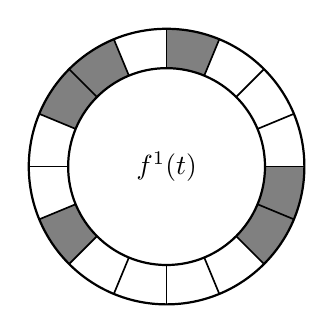
\begin{tikzpicture}[>=latex,font=\sffamily,semithick,scale=1.75]
        \fill [gray] (0,0) -- (90.0:1) arc [end angle=67.5, start angle=90.0, radius=1] -- cycle;
        \fill [white] (0,0) -- (67.5:1) arc [end angle=45.0, start angle=67.5, radius=1] -- cycle;
        \fill [white] (0,0) -- (45.0:1) arc [end angle=22.5, start angle=45.0, radius=1] -- cycle;
        \fill [white] (0,0) -- (22.5:1) arc [end angle=0.0, start angle=22.5, radius=1] -- cycle;
        \fill [gray] (0,0) -- (0.0:1) arc [end angle=-22.5, start angle=0.0, radius=1] -- cycle;
        \fill [gray] (0,0) -- (-22.5:1) arc [end angle=-45.0, start angle=-22.5, radius=1] -- cycle;
        \fill [white] (0,0) -- (-45.0:1) arc [end angle=-67.5, start angle=-45.0, radius=1] -- cycle;
        \fill [white] (0,0) -- (-67.5:1) arc [end angle=-90.0, start angle=-67.5, radius=1] -- cycle;
        \fill [white] (0,0) -- (-90.0:1) arc [end angle=-112.5, start angle=-90.0, radius=1] -- cycle;
        \fill [white] (0,0) -- (-112.5:1) arc [end angle=-135.0, start angle=-112.5, radius=1] -- cycle;
        \fill [gray] (0,0) -- (-135.0:1) arc [end angle=-157.5, start angle=-135.0, radius=1] -- cycle;
        \fill [white] (0,0) -- (-157.5:1) arc [end angle=-180.0, start angle=-157.5, radius=1] -- cycle;
        \fill [white] (0,0) -- (-180.0:1) arc [end angle=-202.5, start angle=-180.0, radius=1] -- cycle;
        \fill [gray] (0,0) -- (-202.5:1) arc [end angle=-225.0, start angle=-202.5, radius=1] -- cycle;
        \fill [gray] (0,0) -- (-225.0:1) arc [end angle=-247.5, start angle=-225.0, radius=1] -- cycle;
        \fill [white] (0,0) -- (-247.5:1) arc [end angle=-270.0, start angle=-247.5, radius=1] -- cycle;
        \draw [thick] (0,0) circle (1);
        \foreach \angle in {90,67.5,...,-67.5}
        \draw (\angle:1) -- (\angle-180:1);
        \node [circle,thick,fill=white,draw=black,align=center,minimum size=2.5cm] at (0,0) {$f^1(t)$};
        \end{tikzpicture} &
        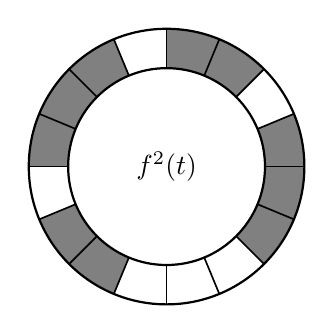
\begin{tikzpicture}[>=latex,font=\sffamily,semithick,scale=1.75]
        \fill [gray] (0,0) -- (90.0:1) arc [end angle=67.5, start angle=90.0, radius=1] -- cycle;
        \fill [gray] (0,0) -- (67.5:1) arc [end angle=45.0, start angle=67.5, radius=1] -- cycle;
        \fill [white] (0,0) -- (45.0:1) arc [end angle=22.5, start angle=45.0, radius=1] -- cycle;
        \fill [gray] (0,0) -- (22.5:1) arc [end angle=0.0, start angle=22.5, radius=1] -- cycle;
        \fill [gray] (0,0) -- (0.0:1) arc [end angle=-22.5, start angle=0.0, radius=1] -- cycle;
        \fill [gray] (0,0) -- (-22.5:1) arc [end angle=-45.0, start angle=-22.5, radius=1] -- cycle;
        \fill [white] (0,0) -- (-45.0:1) arc [end angle=-67.5, start angle=-45.0, radius=1] -- cycle;
        \fill [white] (0,0) -- (-67.5:1) arc [end angle=-90.0, start angle=-67.5, radius=1] -- cycle;
        \fill [white] (0,0) -- (-90.0:1) arc [end angle=-112.5, start angle=-90.0, radius=1] -- cycle;
        \fill [gray] (0,0) -- (-112.5:1) arc [end angle=-135.0, start angle=-112.5, radius=1] -- cycle;
        \fill [gray] (0,0) -- (-135.0:1) arc [end angle=-157.5, start angle=-135.0, radius=1] -- cycle;
        \fill [white] (0,0) -- (-157.5:1) arc [end angle=-180.0, start angle=-157.5, radius=1] -- cycle;
        \fill [gray] (0,0) -- (-180.0:1) arc [end angle=-202.5, start angle=-180.0, radius=1] -- cycle;
        \fill [gray] (0,0) -- (-202.5:1) arc [end angle=-225.0, start angle=-202.5, radius=1] -- cycle;
        \fill [gray] (0,0) -- (-225.0:1) arc [end angle=-247.5, start angle=-225.0, radius=1] -- cycle;
        \fill [white] (0,0) -- (-247.5:1) arc [end angle=-270.0, start angle=-247.5, radius=1] -- cycle;
        \draw [thick] (0,0) circle (1);
        \foreach \angle in {90,67.5,...,-67.5}
        \draw (\angle:1) -- (\angle-180:1);
        \node [circle,thick,fill=white,draw=black,align=center,minimum size=2.5cm] at (0,0) {$f^2(t)$};
        \end{tikzpicture}
    \end{tabular}\\

    \noindent Now suppose you are a xenobiologist exploring $\mathcal{U}: \{\square,\greysquare\}^{128}$, assigned with the task of discovering alien life forms inhabiting in this strange universe. \\

    \noindent (a) Find an \textit{uroboros}, a creature which is its own ancestor: $f^k(\sigma) = \sigma \neq f(\sigma)$.\\
    \noindent (b) Find an \textit{orphan}, a creature which has no parent: $\sigma \in \mathcal{U}  \mid \nexists \sigma'.f(\sigma') = \sigma $.\\
    \noindent (c) Find an \textit{endling}, the last living descendent of its kind: $t \neq f^1(t) = f^2(t)$.\\
    \noindent (d) Find a \textit{chimera}, a creature with three parents: $r, s, t \mid f(r) = f(s) = f(t)$.\\

    \noindent For identification purposes, you may label your specimens for submission using a string of 0s and 1s. Rare and fantastic specimens with additional structure will receive special handling and may be elligible for public viewing.\\

    \noindent \textbf{Bonus} (10 points): Find or design intelligent life in $\mathcal{M}$. This creature should encode a learning algorithm, e.g., a neural network. You must describe the encoding and decoding scheme and demonstrate the creature can learn.\\

    \noindent Please submit your answers as a PDF and supplemental work as a ZIP file.
\end{document}